\documentclass[12pt]{article}
\setlength\parindent{0pt}
\usepackage{fullpage}
\usepackage{graphicx}
\usepackage{amsmath}
\usepackage{color}
\setlength{\parskip}{4mm}
\def\LL{\left\langle}   % left angle bracket
\def\RR{\right\rangle}  % right angle bracket
\def\LP{\left(}         % left parenthesis
\def\RP{\right)}        % right parenthesis
\def\LB{\left\{}        % left curly bracket
\def\RB{\right\}}       % right curly bracket
\def\PAR#1#2{ {{\partial #1}\over{\partial #2}} }
\def\PARTWO#1#2{ {{\partial^2 #1}\over{\partial #2}^2} }
\def\PARTWOMIX#1#2#3{ {{\partial^2 #1}\over{\partial #2 \partial #3}} }
\newcommand{\BE}{\begin{displaymath}}
\newcommand{\EE}{\end{displaymath}}
\newcommand{\BNE}{\begin{equation}}
\newcommand{\ENE}{\end{equation}}
\newcommand{\BEA}{\begin{eqnarray}}
\newcommand{\EEA}{\nonumber\end{eqnarray}}
\newcommand{\EL}{\nonumber\\}
\newcommand{\la}[1]{\label{#1}}
\newcommand{\ie}{{\em i.e.\ }}
\newcommand{\eg}{{\em e.\,g.\ }}
\newcommand{\cf}{cf.\ }
\newcommand{\etc}{etc.\ }
\newcommand{\Tr}{{\rm tr}}
\newcommand{\etal}{{\it et al.}}
\newcommand{\OL}[1]{\overline{#1}\ } % overline
\newcommand{\OLL}[1]{\overline{\overline{#1}}\ } % double overline
\newcommand{\OON}{\frac{1}{N}} % "one over N"
\newcommand{\OOX}[1]{\frac{1}{#1}} % "one over X"
\definecolor{Red}{rgb}{0.8,0,0}
\definecolor{Black}{rgb}{0,0,0}
\newcommand{\black}{\color{Black}}
\newcommand{\red}{\color{Red}}


\begin{document}
\Large
\centerline{\sc{Extra Credit 1: Problems}}
\normalsize
\centerline{\sc{Due Friday, May 5, to your TA's mailbox}}

{\bf Note:} You may do either this assignment or Extra Credit 2, but not both.

{\bf Note 2:} In order to get credit for these problems, you must include text describing your reasoning. All of these problems are difficult; discuss briefly what the difficulty is with each one, and 
how you overcame it. All solutions must be well-reasoned and show all steps.

You can earn up to 0.5 points on your course average per problem, for a maximum of 3.5 points.


\begin{enumerate}

\item In a rotary clothes dryer, sometimes you see a sock move as shown. As the dryer turns (counterclockwise, here), the sock sticks to the wall for a little while,
then -- at some point -- falls off of the wall and lands back on the bottom. If the radius of the dryer is $r$ and it spins at angular velocity $\omega$, find the angle
$\theta$ above the horizontal where it loses contact with the wall.

\begin{center}
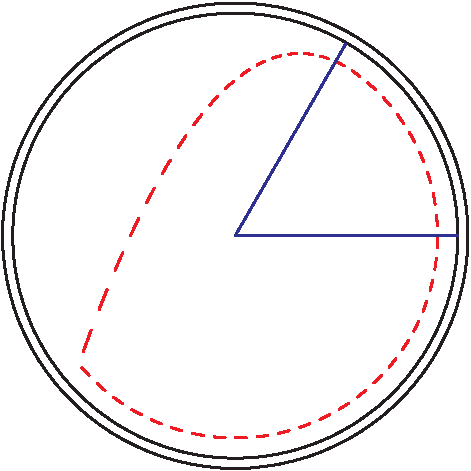
\includegraphics[width=0.5\textwidth]{sock-crop.pdf}
\end{center}


\color{Red}

The sock falls off of the wall when the normal force is zero. This means there is no friction, so the only force
we need to think about is gravity. The radial component of $\vec F_g$ is $mg \sin \theta$; Newton's second
law then gives us 

$$mg \sin \theta = m\omega^2 r$$

which tells us that

$$\theta = \sin^{-1} \frac{\omega^2 r}{g}.$$

\color{Black}

\item An untrained bowler doesn't put any spin on the ball -- he just throws the ball down the lane. Suppose that the ball (moment of inertia $\frac{2}{5}mr^2$)
begins its motion moving at speed $v$, but with $\omega_0 = 0$. Gradually, friction will make the ball start rotating.
If the coefficient of kinetic friction between the ball and the lane is $\mu_k$, how long does it take
for the ball to begin rolling without slipping?

\color{Red}

To make everything positive, imagine the ball going to the left, which we call the positive direction.

$F=ma$ in the $x-$direction tells us that

$$a = -\mu_k g$$

while $\tau = I \alpha$ tells us that

$$\mu_k mgr = \frac{2}{5}mr^2\alpha \rightarrow \alpha = \frac{5}{2} \frac{\mu_k g}{r}$$.

We {\it cannot} set $\alpha r = a$ here, since the ball is not rolling without slipping at first. Instead,
we calculate $\omega(t)$ and $v(t)$ and see at what point $\omega r = v$.

\begin{align}
v(t) &= v_0 - \mu_k gt\\
\omega(t) &= \frac{5}{2} \frac{\mu_k g}{r} t
\end{align}

Setting $v=\omega r$ and solving for $t$ gives us

$$t = \frac{2}{7} \frac{v_0}{\mu_k g}.$$

\color{Black}

\item Two buckets of masses $m_1$ and $m_2$ are connected to a string which hangs over a cylindrical pulley of mass $m_3$. Find the acceleration of the buckets.

\color{Red}

This is a standard Atwood machine; I don't really need to show all the steps, I imagine. The answer is

$$a = \pm \frac{m_1 g - m_2 g}{m_1 + m_2 + \frac{1}{2}m_3}.$$

\color{Black}


\item Suppose that you attach a string to a rock and are whirling it around in a circle. (You may neglect gravity for this problem, so the only force on the rock is the tension of the string.)
Initially, the string has a length $R$ and angular velocity $\omega$.
\begin{enumerate}
\item Suppose that you shorten the string so that it is now length $R/2$. Find the new value of $\omega$.
\item By how much did the kinetic energy change in this process?
\item If the kinetic energy changed, show that this is consistent with the work-energy theorem, $\Delta KE = \int \vec F \cdot d\vec s$. (First, you will need to think about what ``force'' we are talking about here.)
\end{enumerate}

\color{Red}

\begin{enumerate}

\item Conservation of angular momentum tells us pretty trivially that $\omega_f = 4\omega_0$.
\item Just subtract:

$$\Delta KE = \frac{1}{2} I_f \omega_f^2 - \frac{1}{2} I_0 \omega_0^2 = 
\frac{1}{2} m\left(\frac{L}{2}\right)^2 (4 \omega_0)^2 - \frac{1}{2} mL^2 \omega_0^2 = \frac{3}{2} mL^2 \omega_0^2.$$

\item The kinetic energy comes from the required work done. If we imagine pulling the string in very slowly
so that the radial velocity is small throughout, $W = \int\,F_c\,dr$.

This gives us:

$$W = \int_R^{R/2}\,m\omega(r)^2 r\,dr.$$

We note that $\omega(r) = \frac{\omega_0L^2}{r^2}$ by conservation of angular momentum. Substituting this in
we have:

$$W = \int_L^{L/2}\,m\frac{\omega_0^2L^4}{r^4} r\,dr = \omega_0^2L^4 \int_L^{L/2}\,r^{-3}\,dr = 
-\frac{1}{2}\omega_0^2L^4r^{-2}\Big\rvert_L^{L/2}$$

which evaluates to

$$W = \frac{3}{2} mL^2 \omega_0^2$$

consistent with the work-energy theorem, $W = \Delta KE$.

\end{enumerate}
\black
\item A certain car has a maximum engine power of 100 kW and a mass of 1000 kg. The coefficient of static friction between the tires and the pavement is 0.8. The driver of this car wants to accelerate from a stop to 
30 m/s as quickly as possible. (You may neglect air resistance.) How long does this take? (Note: I gave you both the engine power and the coefficient of friction. You need both for your answer; you will need to think about why.)

\red

This problem requires some thought. The maximum traction force might be limited by two things:

\begin{itemize}
\item the available engine power, which imposes a limit $F_{\rm max} = P_{\rm max}/v$, and thus a maximum 
acceleration $a_{\rm max} = P_{\rm max}/(mv)$;
\item the maximum force of static friction, which imposes a maximum acceleration of $\mu_s g$.
\end{itemize}

At low speed, static friction is the limiting factor. At high speed, the engine is the limiting factor.
The transition happens when $$P_{\rm max}/(mv) = \mu_s g \rightarrow v_t = \frac{P_{\rm max}}{\mu_s m g}.$$

It takes a time

$$t_1 = \frac{v_t}{\mu_s g} = \frac{P_{\rm max}}{m \mu_s^2 g^2}$$

for the car to accelerate from a stop to $v_t$. 

To accelerate from $v_c$ to $v_f$, we could deal with the differential equation given by $a(v)$, but 
fortunately there is an easier way. We know that during that period the engine adds power at a rate $P_{\rm max}$,
and the total amount of energy to be added is $\frac{1}{2}mv_f^2 - \frac{1}{2}mv_t^2$.

This means that

$$t_2 = \frac{\frac{1}{2}mv_f^2 - \frac{1}{2}mv_t^2}{P} = \frac{ mv_f^2 - 
\frac{P^2}{\mu_s^2mg^2}}{2P} = 
\frac{mv_f^2}{2P} -\frac{P}{2\mu_s^2mg^2}$$

and the total time is 

$$t_1 + t_2 = \frac{mv_f^2}{2P} + \frac{P}{2\mu_s^2mg^2}.$$

\black

\item A jet-powered sled has a motor that takes a little while to warm up. For the first moments of its ignition, the force it exerts is $F=\beta t$, where $\beta$ is some constant. The coefficients of static and kinetic
friction between the sled and the ground are $\mu_s$ and $\mu_k$, respectively; the sled's mass is $m$. 

\begin{enumerate}
\item How long will it take for the sled to start moving?
\item Write down a (piecewise-defined, if necessary) function for the sled's position as a function of time. 
\end{enumerate}

\red

It starts moving after a time $t_1 = \mu_s mg/\beta$.

After it starts moving, its acceleration is $a(t) = \beta t - \frac{\mu_k mg}{m}$.

In the discussion that follows, define $\tau$ as the time elapsed after it starts moving,
i.e. $\tau = t - t_1$. This means that 
$$a(\tau) = \beta \tau/m + (\mu_s - \mu_k) g.$$

If we try to solve this in terms of $t$, then it becomes very difficult to identify what the constants
of integration are. Doing this in terms of $\tau$ makes this easy.

We now simply integrate acceleration twice to get position. The constants of integration are both zero, since
$v(\tau = 0) = a(\tau = 0) = 0$.

\begin{align*}
a(\tau) &= \beta \tau/m + (\mu_s - \mu_k) g \\
v(\tau) &= \frac{1}{2}\beta \tau^2/m + (\mu_s - \mu_k) g \tau \\
x(\tau) &= \frac{1}{6}\beta \tau^3/m + \frac{1}{2}(\mu_s - \mu_k) g \tau^2 \\
\end{align*}

You can substitute $t=\tau + \mu_smg/\beta$ back in to get answers in terms of $t$, or leave it as is.

\black



\item A moon orbits a planet in a circular orbit at distance $r$ and angular velocity $\omega$. An engineer would like to place a satellite somewhere between the moon and the planet so that it, 
also, orbits the planet in a circular orbit with angular velocity $\omega$, synchronized with the orbit of the moon. 

Somewhere between the moon and the planet, at some intermediate radius $R$ between 0 and $r$, there is a point (called a ``Lagrange point''), where this is possible. Find $R$. 


\red

Here the net gravitational force equals $m\omega^2 r$. Thus we have:

$$\omega^2 R = \frac{GM}{R^2} - \frac{GM}{(r-R)^2}$$

This is a cubic equation and doesn't have a simple closed-form solution. Students who recognize this
get full credit (since it could easily be solved numerically). 

\end{enumerate}
\end{document}
